\documentclass[aspectratio=169]{beamer}
\mode<presentation>
%\usetheme{Warsaw}
%\usetheme{Goettingen}
\usetheme{Hannover}
%\useoutertheme{default}

%\useoutertheme{infolines}
\useoutertheme{sidebar}
\usecolortheme{dolphin}


\setbeamersize{sidebar width left=0pt} % to remove the sidebar
\beamertemplatenavigationsymbolsempty % To remove the navigation symbols on the bottom right.
\setbeamersize{text margin left=10mm,text margin right=10mm} % Specify margins

\usepackage{amsmath}
\usepackage{amssymb}
\usepackage{listings}
\usepackage{enumerate}
\usepackage{hyperref}
\hypersetup{
    colorlinks=true,
    linkcolor=blue,
    filecolor=magenta,      
    urlcolor=cyan,
}
 
\urlstyle{same}

%some bold math symbosl
\newcommand{\Cov}{\mathrm{Cov}}
\newcommand{\Var}{\mathrm{Var}}
\newcommand{\brho}{\boldsymbol{\rho}}
\newcommand{\bSigma}{\boldsymbol{\Sigma}}
\newcommand{\btheta}{\boldsymbol{\theta}}
\newcommand{\bbeta}{\boldsymbol{\beta}}
\newcommand{\bmu}{\boldsymbol{\mu}}
\newcommand{\bW}{\mathbf{W}}
\newcommand{\one}{\mathbf{1}}
\newcommand{\bH}{\mathbf{H}}
\newcommand{\by}{\mathbf{y}}
\newcommand{\bolde}{\mathbf{e}}
\newcommand{\bx}{\mathbf{x}}

\newcommand{\cpp}[1]{\texttt{#1}}

%--------------------------------------------------
\providecommand{\abs}[1]{\lvert#1\rvert}
\providecommand{\norm}[1]{\lVert#1\rVert}
\providecommand{\Blue}[1]{\textcolor{blue}{#1}}
\providecommand{\Red}[1]{\textcolor{red}{#1}}
\newcommand{\celsius}{\ensuremath{^\circ}C}
\newcommand\thfore{\mathord{\therefore}\,}
%------------------------------------------------------------------

\title{Lecture 27. Basics Counting Operations in Algorithms II}

%\author{\includegraphics[width=.7\textwidth,height=.7\textheight]{lecture20-fig0.png}}

\date{ }
\vspace{.5in}

%------------------------------------------------------------------


\begin{document}

\frame[plain]{\titlepage}


\begin{frame}[plain]{ }

 {\bf Example 27.1}. Consider the recursive binary search algorithm
		   
		   \begin{center}
		   	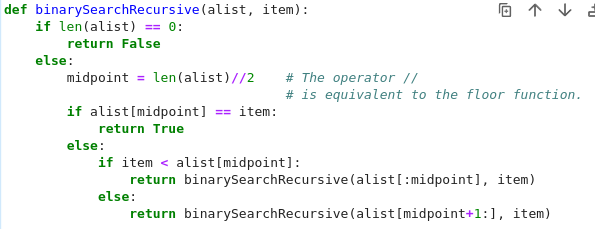
\includegraphics[height=4cm]{./img/lecture27-fig1.png}
		   \end{center}
		   
  \begin{itemize}
   \item[(a)]  Let $X = \{ 2, 3, 5, 8, 13, 21, 34, 55, 70 \}$. Evaluate 
  $ \mathrm{binarySearchRecursive(X, 55)}. $  
  \item[(b)] Find a recurrence relation of counting  number of comparisons in the algorithm
  \item[(c)]  Use (b) to approximate the worst-case complexity of the recursive binary search function.
  \end{itemize}
  
  %finalF15
    %Lecture25 Exercise
    %Exam2S23
    
    \vspace{.5in} 
	
\end{frame}

%\begin{frame}[plain]{}

% {\bf Activity 20.2}. What will be the value '\texttt{\Blue{counter}(10, 9,  7, 10, 5)}' 
% when the following code is run?
    
%    \begin{center}
%			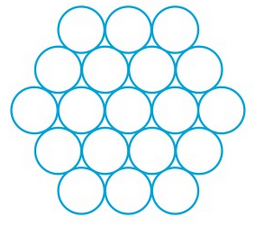
\includegraphics[height=4cm]{lecture20-fig3.png} 
%	\end{center}
	
	
%	\vspace{.5in}
	
%\end{frame}


%%%%%%%%%%%%%%%%%%
\iffalse
\begin{frame}[plain]{Counting}

{\bf Activity 20.1}. How many bit strings of length four start with 1 or end with 00?
 %https://ggc-discrete-math.github.io/counting.html#_counting    Example 7

\vspace{2.5in}

\end{frame}

\fi
%%%%%%%%%%%%%%%%%%%%%%%%%%%%
 


 
\end{document}

%%%%%%%%%%%%%%%%%%%%%%%%%%%%%%%%%%%%%%%%%%%%%%%%%%%

\begin{frame}[plain]{Exercises}

  \begin{enumerate}
   \item A startup with four employee rents an office suite with seven offices. 
    How many ways are there to assign the employees?
   \item Let $n>3$. Consider the following pseudocode segment.
   
       \begin{center}
			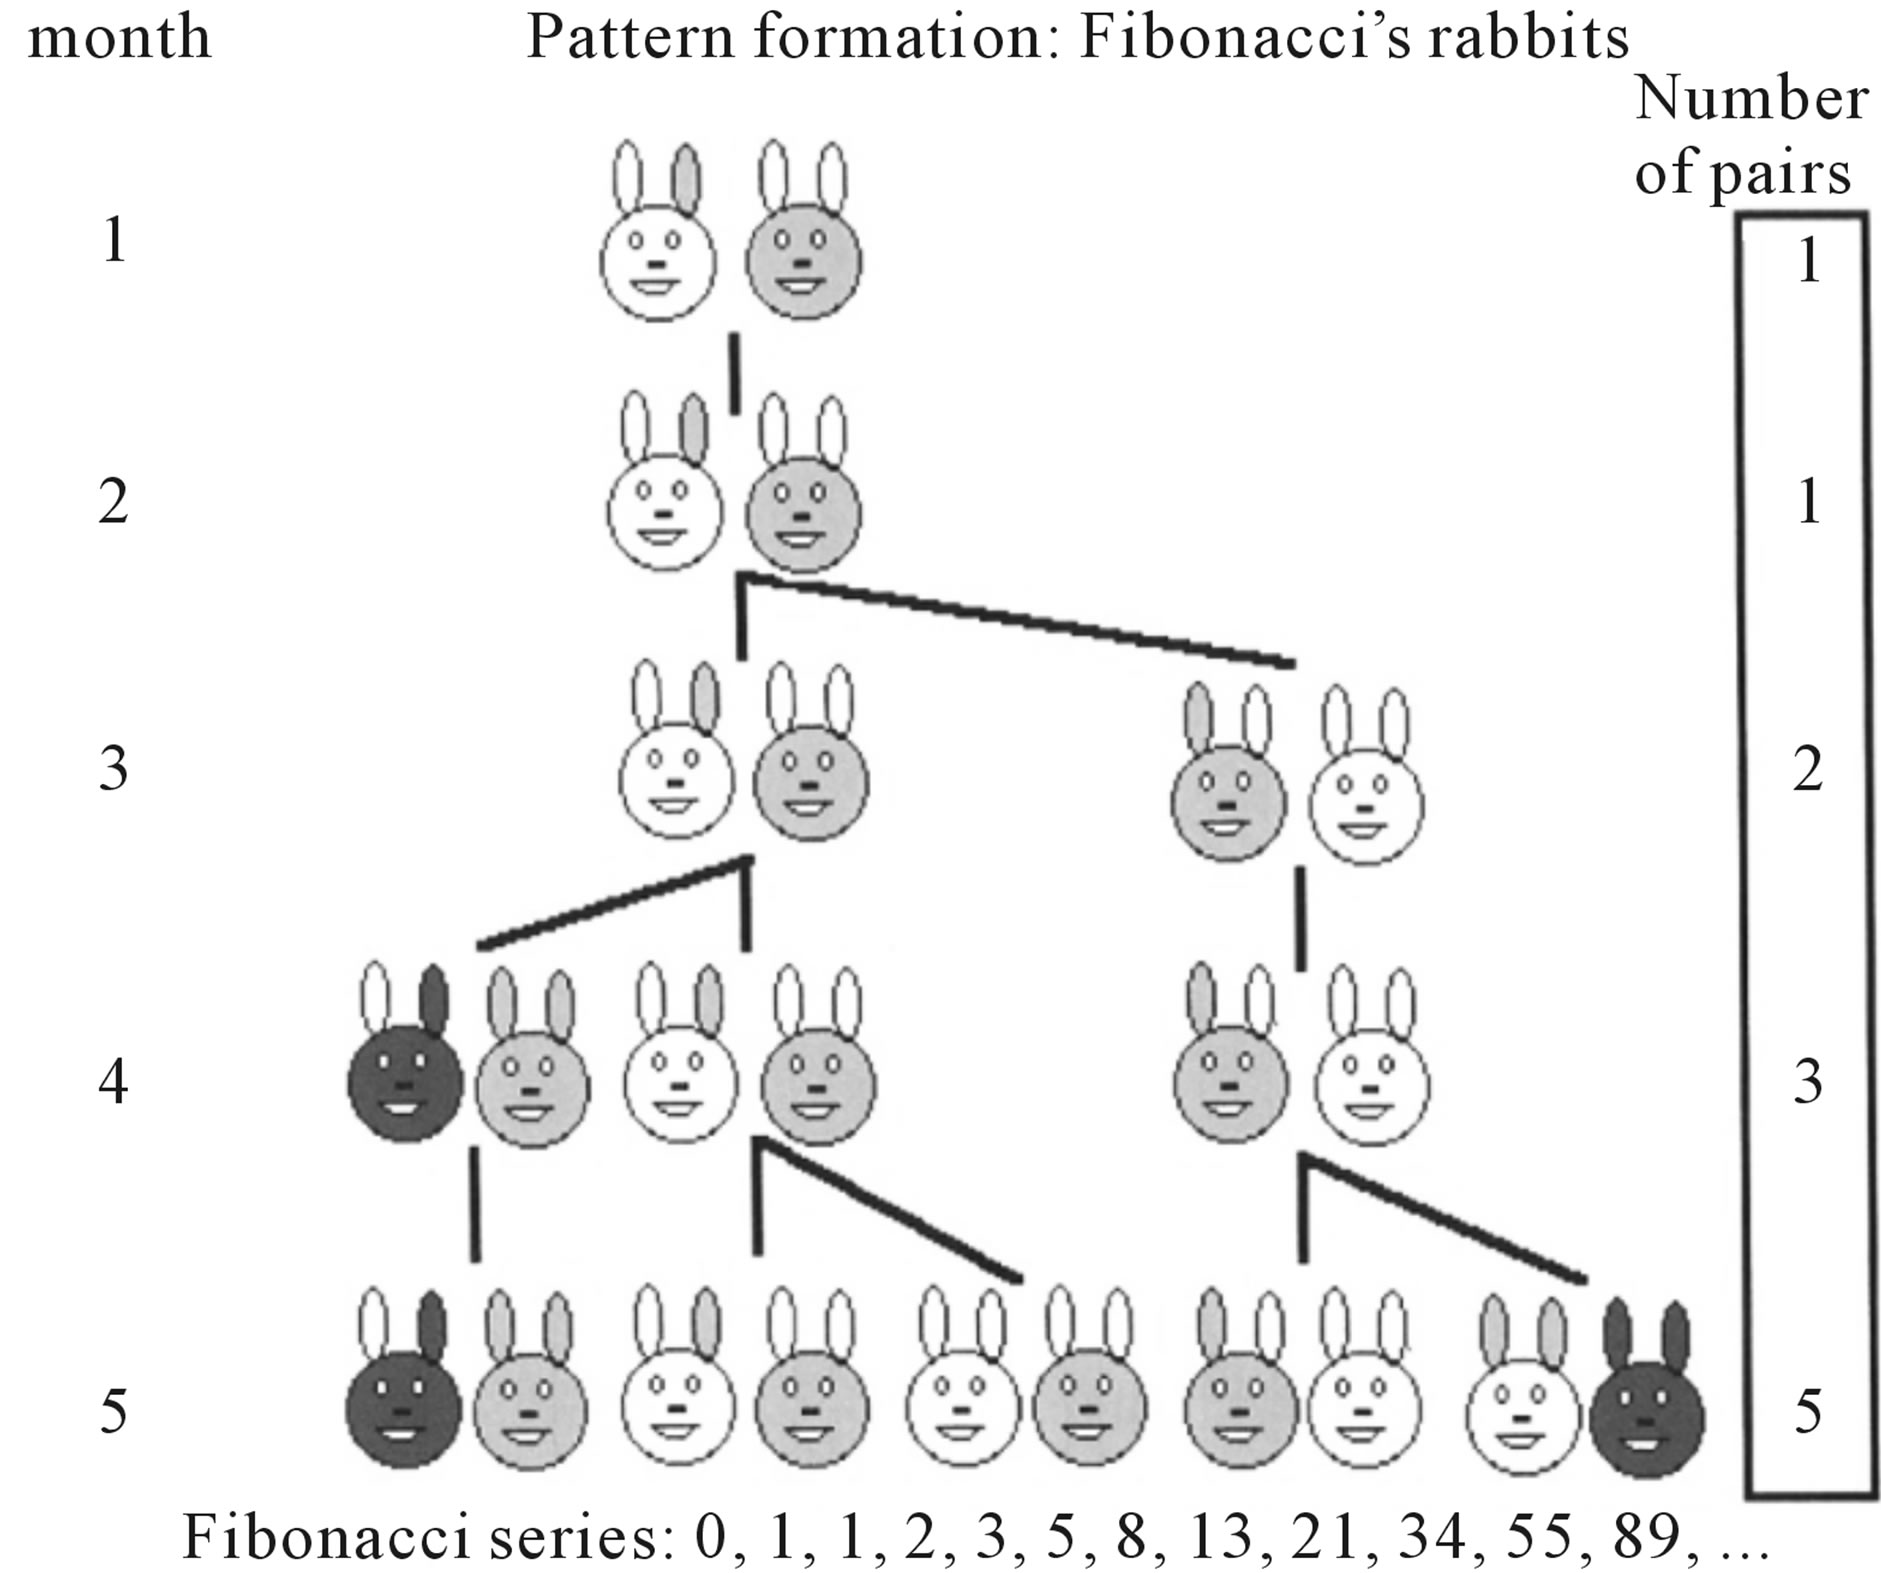
\includegraphics[height=3.3cm]{lecture20-fig1.png}
		\end{center}
		How many "+" operations does this algorithm perform?
		%Essentials (3rd), Exercises 4.5 #11 on p280
   \item If a card is drawn from a standard 52-card deck,
    how many ways can the card be black or a face card?

  \end{enumerate}

\end{frame}

\begin{frame}[plain]{}

  \begin{enumerate}
   \setcounter{enumi}{3}

  \item Let $x_1, x_2, ..., x_n$ be an array whose elements can be compared 
    by the total ordering $\leq$. 
    \begin{itemize}
      \item[(a)] Write an algorithm for computing the maximum element in the array. 
      \item[(b)] How many ``$<$" comparisons does your algorithm require?
      \item[(c)] Write a python code based on your algorithm and test your assertion in (b) with   
    examples of several arrays.
   \end{itemize}
    %https://github.com/bkimo/discrete-math-with-python/blob/master/lab2-bubble-sort.ipynb
  \end{enumerate}

\end{frame}








\end{document}

